\chapter{\sysname Feedback from Study Participants}
\label{app-feedback}

As part of the post-conversation survey described in \cref{ch:mibot-eval}, participants responded to the following three feedback questions:

\begin{tcolorbox}[breakable,
		% width=\textwidth, % Full page width
		colback=magenta!5!blue!10,        % Light pink/purple background
		colframe=magenta!60!blue!40,      % Darker purple/pink frame
		fonttitle=\bfseries, % Bold title font
		fontupper=\small,
		%title=Prompt for Virtual Smoker Client, % Box title
		title=Feedback Survey Questions]

	\begin{enumerate}
		\item What are three words that you would use to describe the chatbot?
		\item What would you change about the conversation?
		\item Did the conversation help you realize anything about your smoking behaviour? Why or why not?
	\end{enumerate}

\end{tcolorbox}



Participant feedback on \sysname was generally positive. We processed the feedback by dividing the words participants used to describe the chatbot into broad \textit{positive} and \textit{negative} categories. The word cloud (\Cref{word_cloud}) represents these words. The top 10 most frequently mentioned positive and negative words are shown in \Cref{tab:top10pos,tab:top10neg}.


\renewcommand{\thetable}{J.\arabic{table}}
\setcounter{table}{0}

\begin{table}[!htpb]
	\centering
	\begin{tabular}{lr}
		\toprule
		\textbf{Word}          & \textbf{Frequency} \\
		\midrule
		\texttt{understanding} & 24                 \\
		\texttt{helpful}       & 22                 \\
		\texttt{friendly}      & 19                 \\
		\texttt{supportive}    & 12                 \\
		\texttt{caring}        & 9                  \\
		\texttt{knowledgeable} & 8                  \\
		\texttt{intelligent}   & 8                  \\
		\texttt{thoughtful}    & 7                  \\
		\texttt{interesting}   & 7                  \\
		\texttt{informative}   & 7                  \\
		\bottomrule
	\end{tabular}
	\caption[Top 10 most frequently mentioned positive words in participant feedback]{Top 10 most frequently mentioned positive words in participant feedback.}
	\label{tab:top10pos}

\end{table}

\vspace{1em}

\begin{table}[!htpb]
	\centering
	\begin{tabular}{lr}
		\toprule
		\textbf{Word}          & \textbf{Frequency} \\
		\midrule
		\texttt{repetitive}    & 6                  \\
		\texttt{boring}        & 3                  \\
		\texttt{unresponsive}  & 1                  \\
		\texttt{disappointing} & 1                  \\
		\texttt{annoying}      & 1                  \\
		\texttt{dull}          & 1                  \\
		\texttt{pointless}     & 1                  \\
		\texttt{useless}       & 1                  \\
		\texttt{uncreative}    & 1                  \\
		\texttt{overbearing}   & 1                  \\
		\bottomrule
	\end{tabular}
	\caption[Top 10 most frequently mentioned negative words in participant feedback]{Top 10 most frequently mentioned negative words in participant feedback.}
	\label{tab:top10neg}

\end{table}



\begin{figure*}[!htbp]
	\centering
	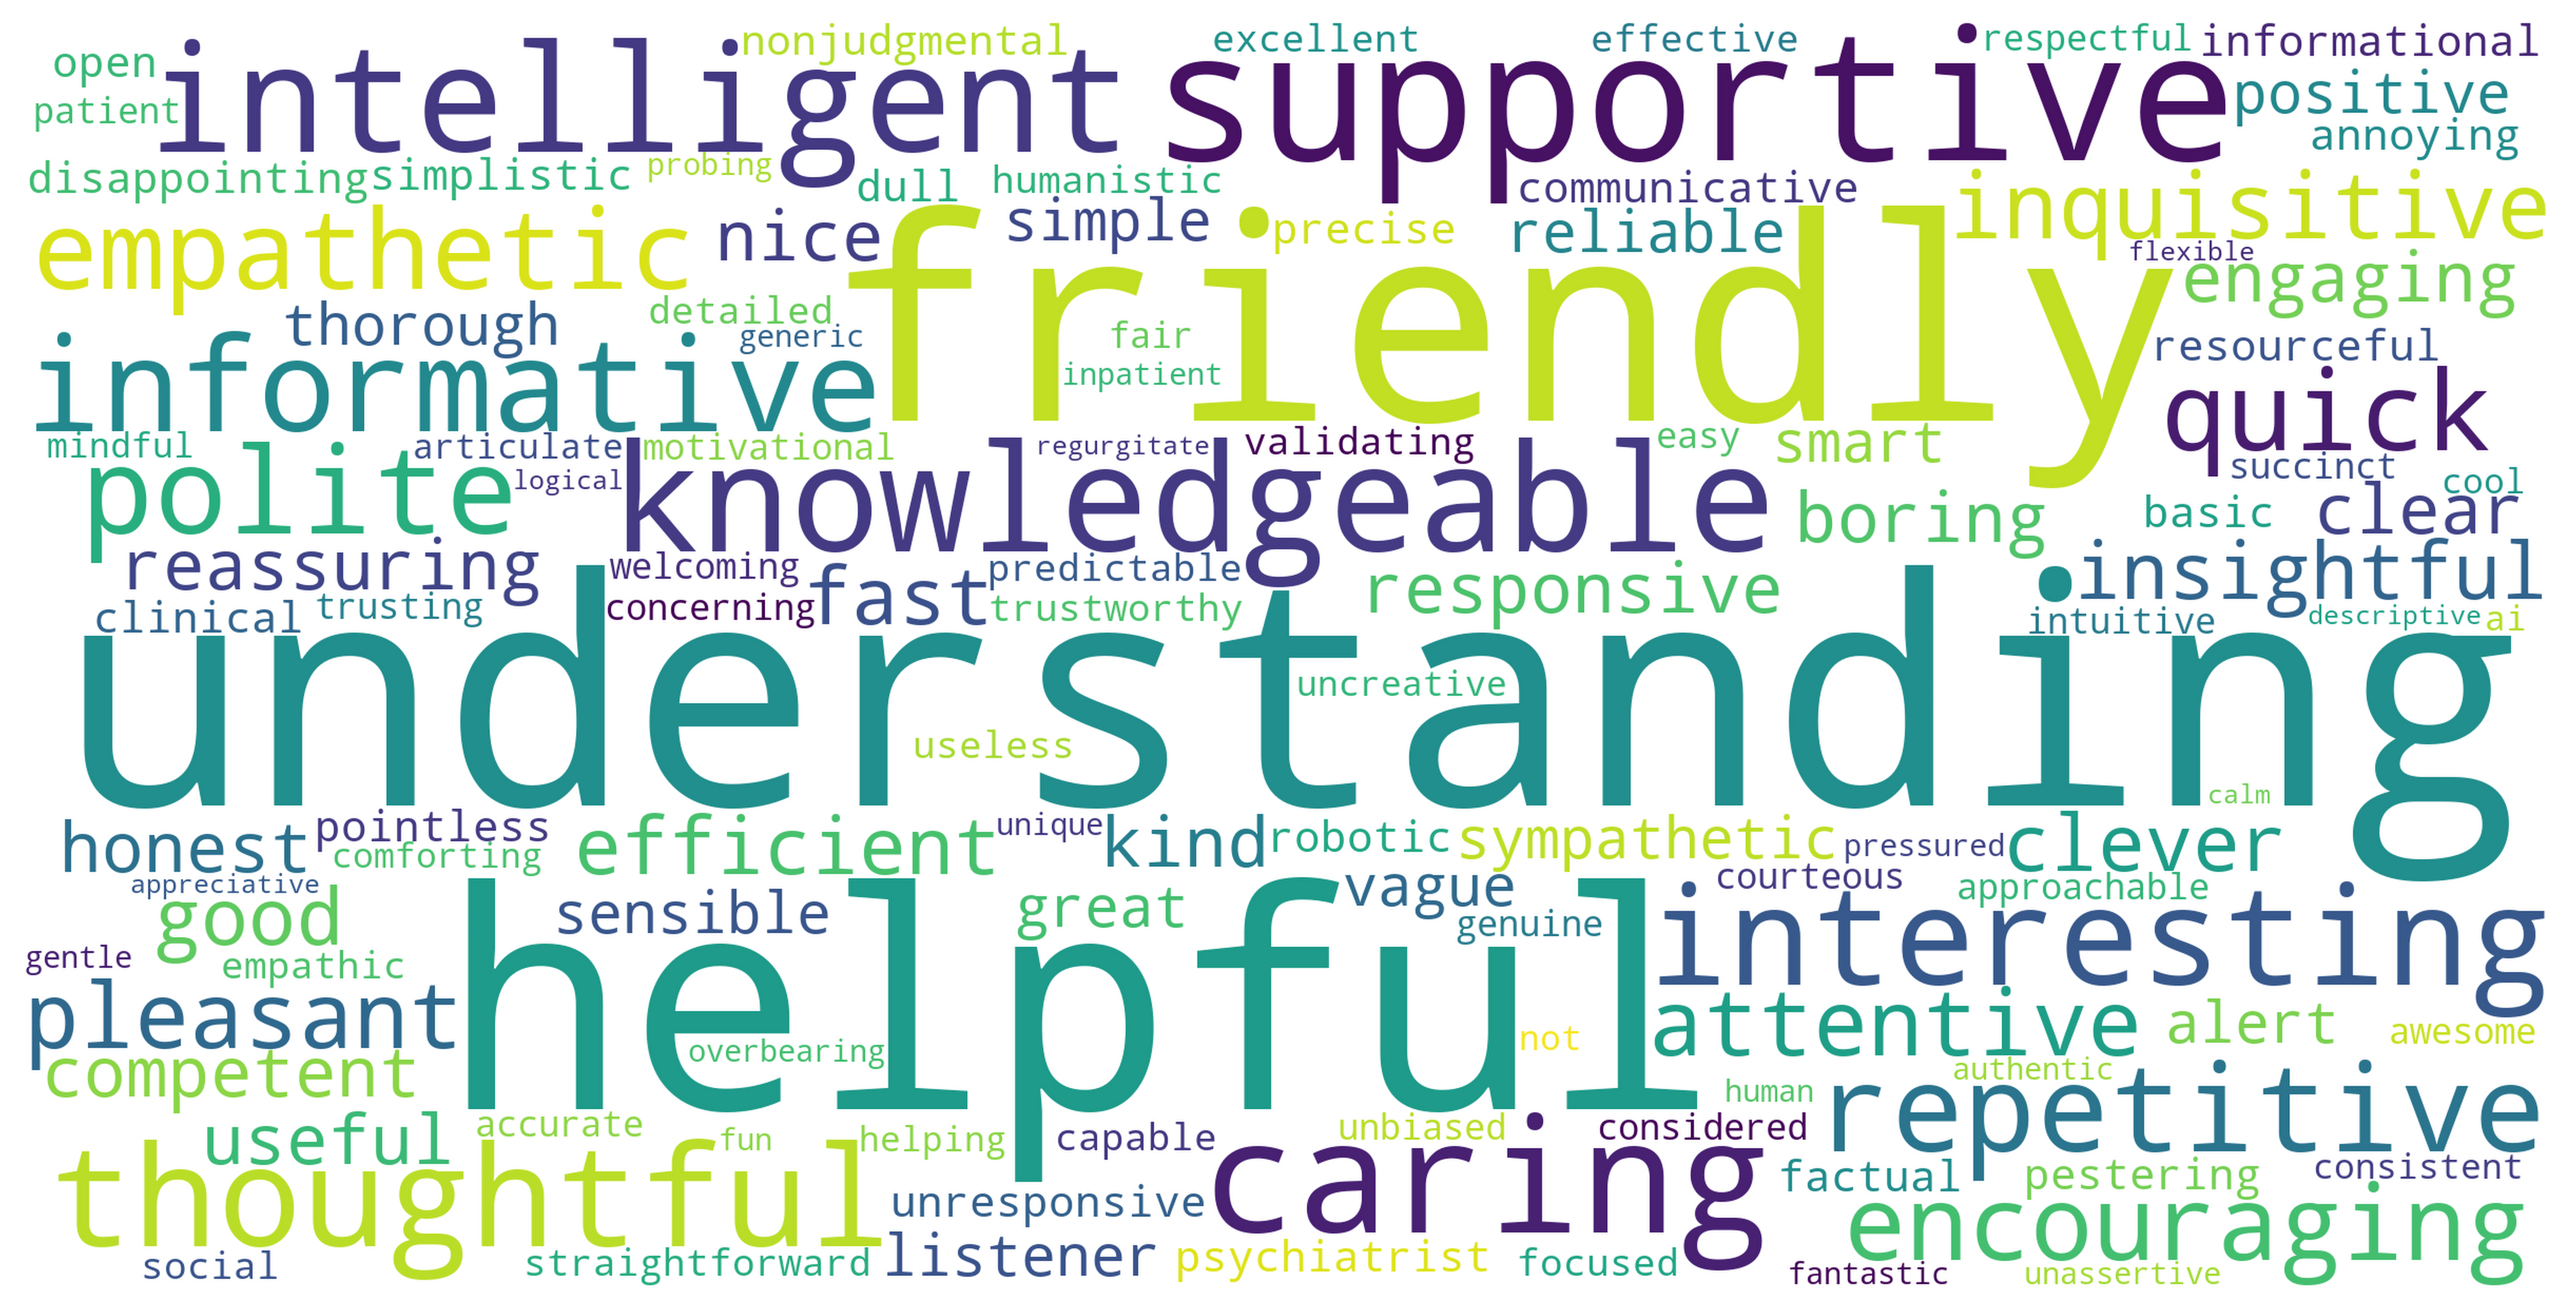
\includegraphics[width=0.9\textwidth]{fig/wordcloud.png}
	\caption[Word cloud representation of participant feedback]{Word cloud representation of participant feedback.}
	\label{word_cloud}
\end{figure*}
